\section{Test af hardware}
\subsection{Modultest}
Før at vi kunne teste det samlede system bestående af både hardware og software, måtte vi foretage nogle modultests af de enkelte dele i hardwaren. Forstærkeren, subtractoren samt filteret er blevet testet på fumlebrættet, og i forbindelse med disse test har vi skiftet mellem at bruge en spændingsdeler og transduceren tilsluttet vandsøjlen. Da testene var godkendt, kunne vi tilkoble alt hardwaren og lave integrationstest.

\subsubsection{Forstærker}
I testene for forstærkeren brugte vi en spændingsdeler, da Analog Discovery ikke kan levere
lave nok spændinger uden alt for meget støj. Vi måtte have en lav spænding, da transducerens
output tilsvarende er en lav spænding. Spændingsdeleren fungerede derfor som en erstatning
af transduceren, hvor vi blot selv kunne bestemme hvilket type signal vi ville sende igennem
forstærkeren.

\textbf{Test med spændningsdeler}

Vi ville teste at signalet blev forstærket 320 gange, hvilket vi gjorde ved at sende 4 V gennem spændingsdeleren samt forstærkeren, og målte på udgangen af forstærkeren. Her forventede vi at få et output på 4 V fra forstærkeren, da spændingsdelerens output var 320 gange mindre end de 4 V. Input til spændningsdeleren og output fra forstærkeren burde være det samme, hvilket stemte overens med vores faktiske resultater.

\textbf{Test med transducer og vandsøjle}

I denne test erstattede vi spændningsdeleren med transduceren, som blev tilsluttet vandsøjlen. Der blev udført en række tests med forskellige tryk på transduceren, for at undersøge om signalet blev forstærket op 320 gange, samt teste lineariteten og nøjagtigheden af vores målinger.
Nedenstående graf repræsenterer testresultaterne fra et tryk på 0, 10, 50 og 100 mmHg.

\vspace{0.5 cm}

\begin{figure}[h!]
	\centering
	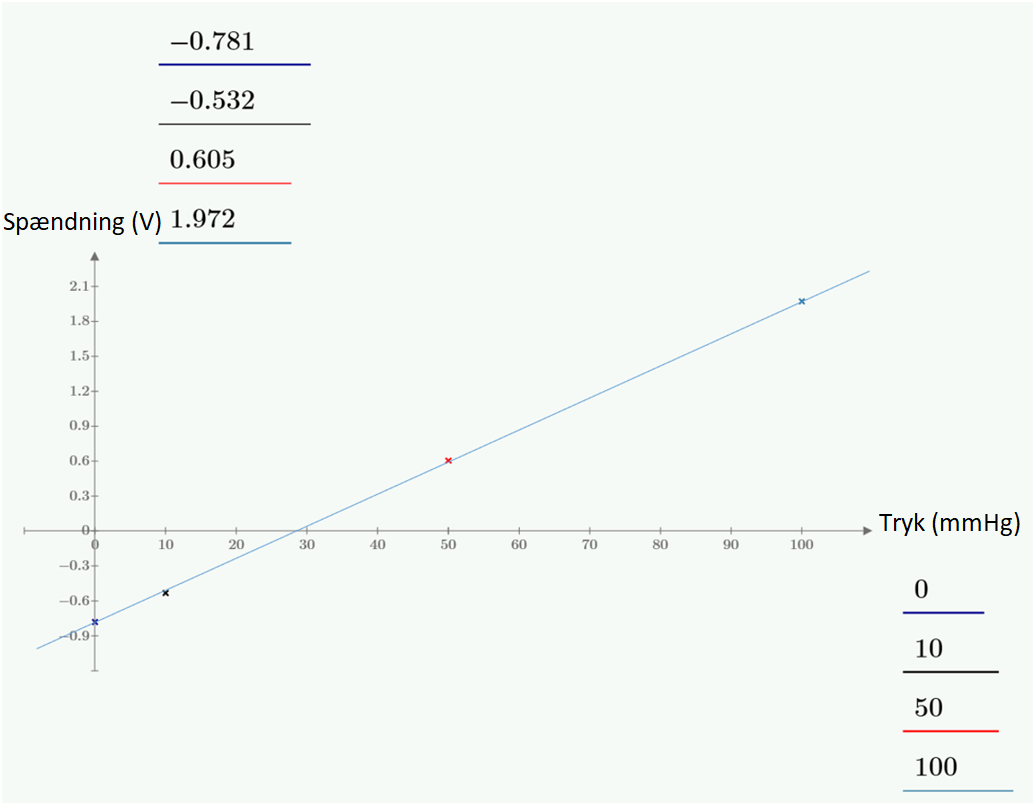
\includegraphics[width=0.6\linewidth]{../Rapport/Implementering_og_test/Hardware/forstaerker}
	\caption{Modultest af forstærker på fumlebræt}
	\label{fig:forstaerker}
\end{figure}

\clearpage

På x-aksen er tryk i mmHg, og på y-asken er spænding i V. Det ses at der er en god lineær sammenhæng mellem tryk og spænding, samt at signalet er blevet forstærket. Da vi på vandsøjlen kun kan måle op til 100 mmHg antager vi at denne sammenhæng fortsætter kan følgende regnestykke opstilles: 

\[\frac{250 mmHg}{100 mmHg} = 2,5 \]
\[ 1,972 V \cdot 2,5 = 4,93 V \]
\[ 4,93 V - 0,781 V = 4,149 V \]

Ud fra tidligere beregninger vil vi forvente at et tryk på 250 mmHg vil have en spænding på 4 V, hvilket stemmer godt overens med vores test. De specifikke måleresultater findes i bilag for test af hardwaren.

\subsubsection{Subtractor}

For at teste subtractoren brugte vi waveforms til at genere to signaler. Et DC-signal på 2 V, hvilket subtractoren bruger til at trække et signal ned med 2 V. Det andet signal var et sinussignal, som blev sendt gennem subtractoren. I testen forventede vi, at subtractoren ville sænke sinussignalet 2 V ned i dens amplitude. Vi sendte et sinussignal ind med et offset på 2 V, for at hæve signalet, som vi derefter vha. subtractoren kunne sænke. Vi målte signalerne ved brug af waveforms scope funktion.

\begin{figure}[h!]
	\centering
	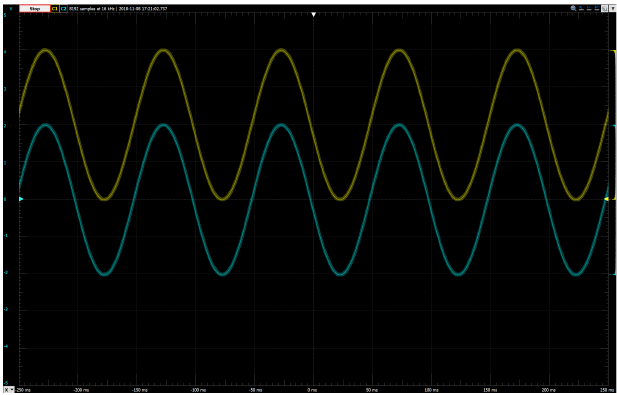
\includegraphics[width=0.72\linewidth]{../Rapport/Implementering_og_test/Hardware/subtractor}
	\caption{Test af subtractor}
	\label{fig:subtractor}
\end{figure}

På ovenstående screenshots ses den gule kurve, som et sinussignal med en amplitude på 2 V og et offset på 2 V. Der benyttes et sinussignal, for at teste subtractorens nedeskalering af forskellige amplituder. Den blå kurve er outputtet fra subtractoren, hvilket har sænket det oprindelige sinussignal med 2 V. Subtractoren virkede derfor som den skulle, i og med at den kunne sænke signalet med de ønskede 2 V.

\clearpage

\subsubsection{Filter}

Da vi testede filteret, sendte vi et sinussignal ind på filteret med en amplitude på 2 V. For at undersøge filtrets dæmpning gav vi signalet 24 forskellige hertz i et range på 10 til 500 Hz. Resultaterne er påvist på nedenstående bodeplot.

\begin{figure}[h!]
	\centering
	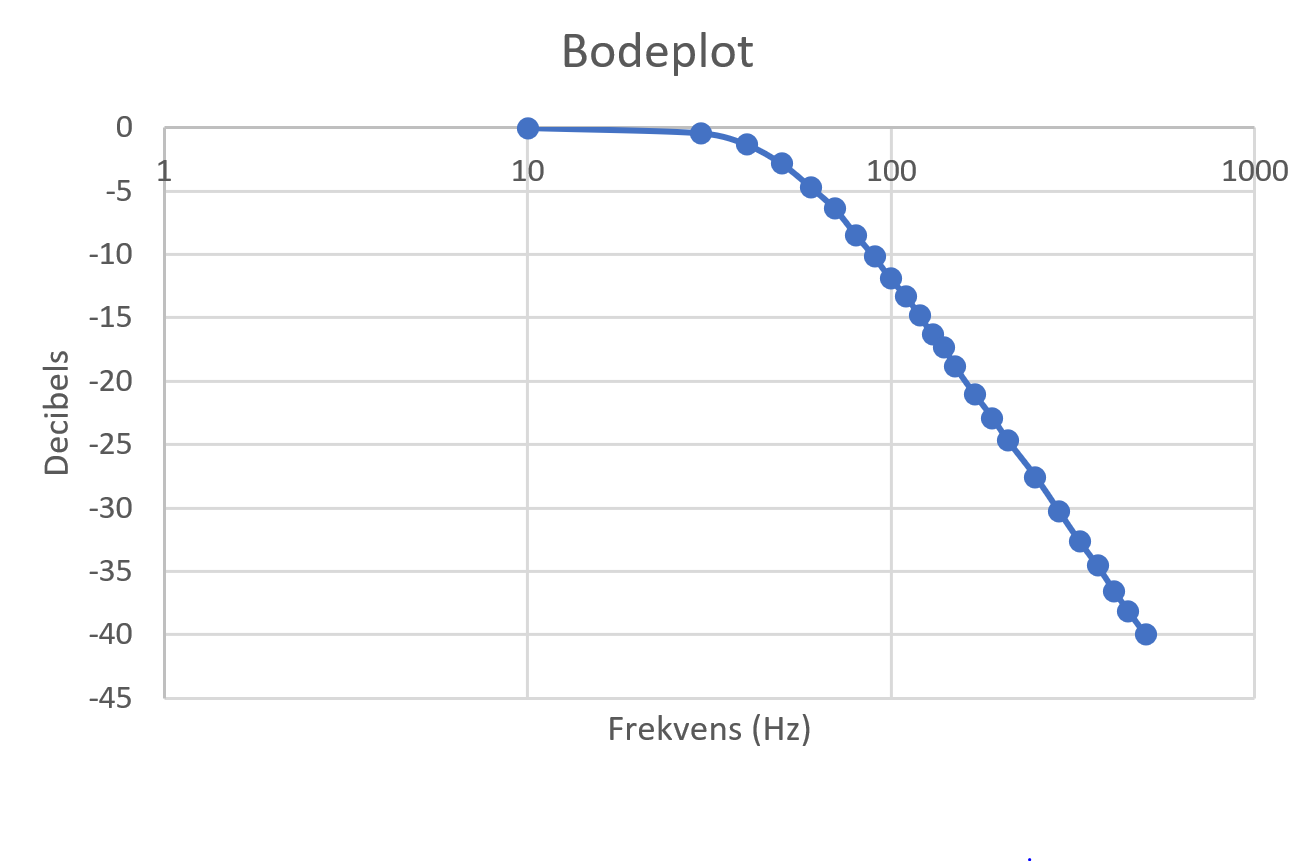
\includegraphics[width=0.8\linewidth]{../Rapport/Implementering_og_test/Hardware/filter}
	\caption{Test af filter}
	\label{fig:filter}
\end{figure}

Det ses at signalet ved 500 Hz dæmper 40 dB pr dekade, hvilket stemmer overens med vores ventede resultat. De specifikke måleværdier kan findes i bilag for test af hardwaren.
Kravet er at filteret skal dæmpe 20 dB over den dekade der er til rådighed, så i teorien har vi ikke brug for et 2. ordensfilter. Dog i tilfælde af at vi brugte 1. ordensfilter, skulle alt performe fuldstændigt perfekt, hvilket var en risiko vi ikke var villige at tage, og derfor benytter vi et 2. ordensfilter.

\clearpage